%%%%
\documentclass[10pt,answers]{exam}
\usepackage{times}
\usepackage{enumerate}
\usepackage{enumitem}
\usepackage{mathtools}
\usepackage{hyperref}
\usepackage{ragged2e}
\usepackage{graphicx}
\usepackage{blindtext}
\usepackage{pgf}
\usepackage{tikz}
\usepackage{caption}
\usepackage{subcaption}
\usepackage{blkarray}
\usepackage{amsfonts}
\usepackage{graphicx}
\usepackage{float}
%Feel free to add packages and newcommands here if you wish
    
%%%%
% IMPORTANT: YOU SHOULD INSTANTIATE THE FOLLOWING THREE COMMANDS WITH YOUR OWN DETAILS
\newcommand{\authorname}{George Theodoridis}     %%% Write your first and last name
\newcommand{\authornumber}{S5951178}  %%% Write your student number
\newcommand{\assignmentnumber}{1}  %%% Write 1, 2, 3, etc
%%%%

%%%% DO NOT MODIFY 

\pagestyle{headandfoot}
\runningheadrule
\firstpageheader{Computer Architecture (2024-2025)}{{\textbf{Assignment}~\assignmentnumber} \\ \today}{}
\runningheader{Individual solutions by \authorname~(\authornumber)}
              {}
              {Page \thepage\ of \numpages}
\firstpagefooter{}{}{}
\runningfooter{}{}{}
\newcommand{\qpoints}[1]{\hfill \textbf{(#1 points)}}
 
\begin{document}
 \boxedpoints
\begin{center}
  \fbox{\fbox{\parbox{0.97\textwidth}{\centering
  {\Large
 \authorname~(\authornumber)  }}}
 }
\end{center}

\begin{enumerate}
\item[] \textbf{INSTRUCTIONS}

\item Submission is only via Brightspace. Deadlines are strict.

\item The exercises in this assignment add up to 100 points. To calculate your grade simply divide the number of points by 10.

\item You must submit a pdf typeset in (La)TeX (no handwritten solutions) using \textbf{this} template.

\item Seeking solutions from the internet, from any external resource, or from any other person is prohibited.

\item Please note that the course lecturer reserves the right to ask the student submitting the assignment to explain the answers to any or all questions. If the student is unable to provide a satisfactory answer then that question may receive partial/no credit. 

\item Of course, university policies on plagiarism always apply. In particular, any suspected plagiarism will be reported to the Board of Examiners.
\end{enumerate}
\rule{6cm}{0.4pt}

\bigskip
\bigskip


%%% MODIFICATIONS ALLOWED FROM HERE

\begin{questions}
\question Convert the following decimal numbers to their 2’s complement representations (use 8 bits for each number and truncate the fractional digits if necessary): \qpoints{10}
\begin{enumerate}[label=\alph*)]
    \item 42.3
    \item 6.3      
    \item -13     
    \item 0.04   
\end{enumerate}

\begin{solution}
\begin{enumerate}[label=\alph*)]
	\item 00101010
	\item 00000110
	\item 11110011
	\item 00000000
\end{enumerate}
\end{solution}

\question Perform the following operation in 2’s complement. Indicate when an overflow happens. \qpoints{10}
\begin{enumerate}[label=\alph*)]
    \item 11001010  + 11101010
    \item 01011010 + 00110101  
    \item 0011.1100 + 0100.0100 
    \item 11010111 – 00001011
\end{enumerate}

\begin{solution}
\begin{enumerate}[label=\alph*)]
	\item 10110100 no overflow
	\item 10001111 overflow
	\item 1000.0000 overflow
	\item 11001100 no overflow
\end{enumerate}
\end{solution}

\newpage
\question Write IEEE floating point representation of the following decimal numbers. \qpoints{10}
\begin{enumerate}[label=\alph*)]
    \item 19.45   
    \item -0.028 
\end{enumerate}

\begin{solution}
	\begin{enumerate}[label=\alph*)]
		\item 0 10000011 00110111001100110011001
		\item 1 01111001 11001010110000001000010
	\end{enumerate}
\end{solution}


\question The following numbers are in IEEE floating point representation. Write their decimal equivalents. \\ \qpoints{10}
\begin{enumerate}[label=\alph*)]
    \item 1 01111001 10101010000000000000000 
    \item 0 00000000 00001000000000000000000
\end{enumerate}


\begin{solution}
	\begin{enumerate}[label=\alph*)]
		\item -0.0260009765625
		\item $3.67341985 * 10^{-40}$
	\end{enumerate}
\end{solution}

\question Design a circuit that outputs a 1 only if exactly two out of three inputs (A, B, C) are 1. (Use only NOT gates or logic gates with 2 inputs.) \qpoints{15}

\begin{solution}
	\begin{figure}[H]
		\centering
		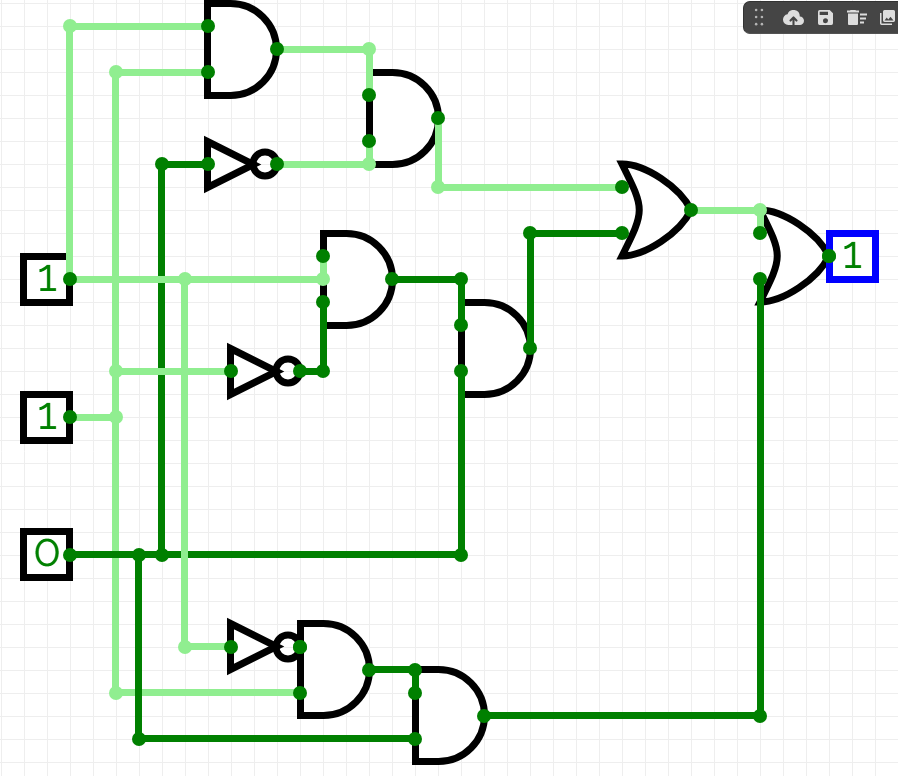
\includegraphics[width=\textwidth]{ex5.png}
		\caption{ex5}
    	\label{fig:ex5}
	\end{figure}
\end{solution}


\question Using a decoder and an encoder, design a circular incrementor circuit for 4-bit positive binary numbers. The input (a number between 0 and 7) will be incremented by one if it is less than 7. If the input is 7, the output should become zero. \qpoints{15}
\begin{solution}
	\begin{figure}[H]
		\centering
		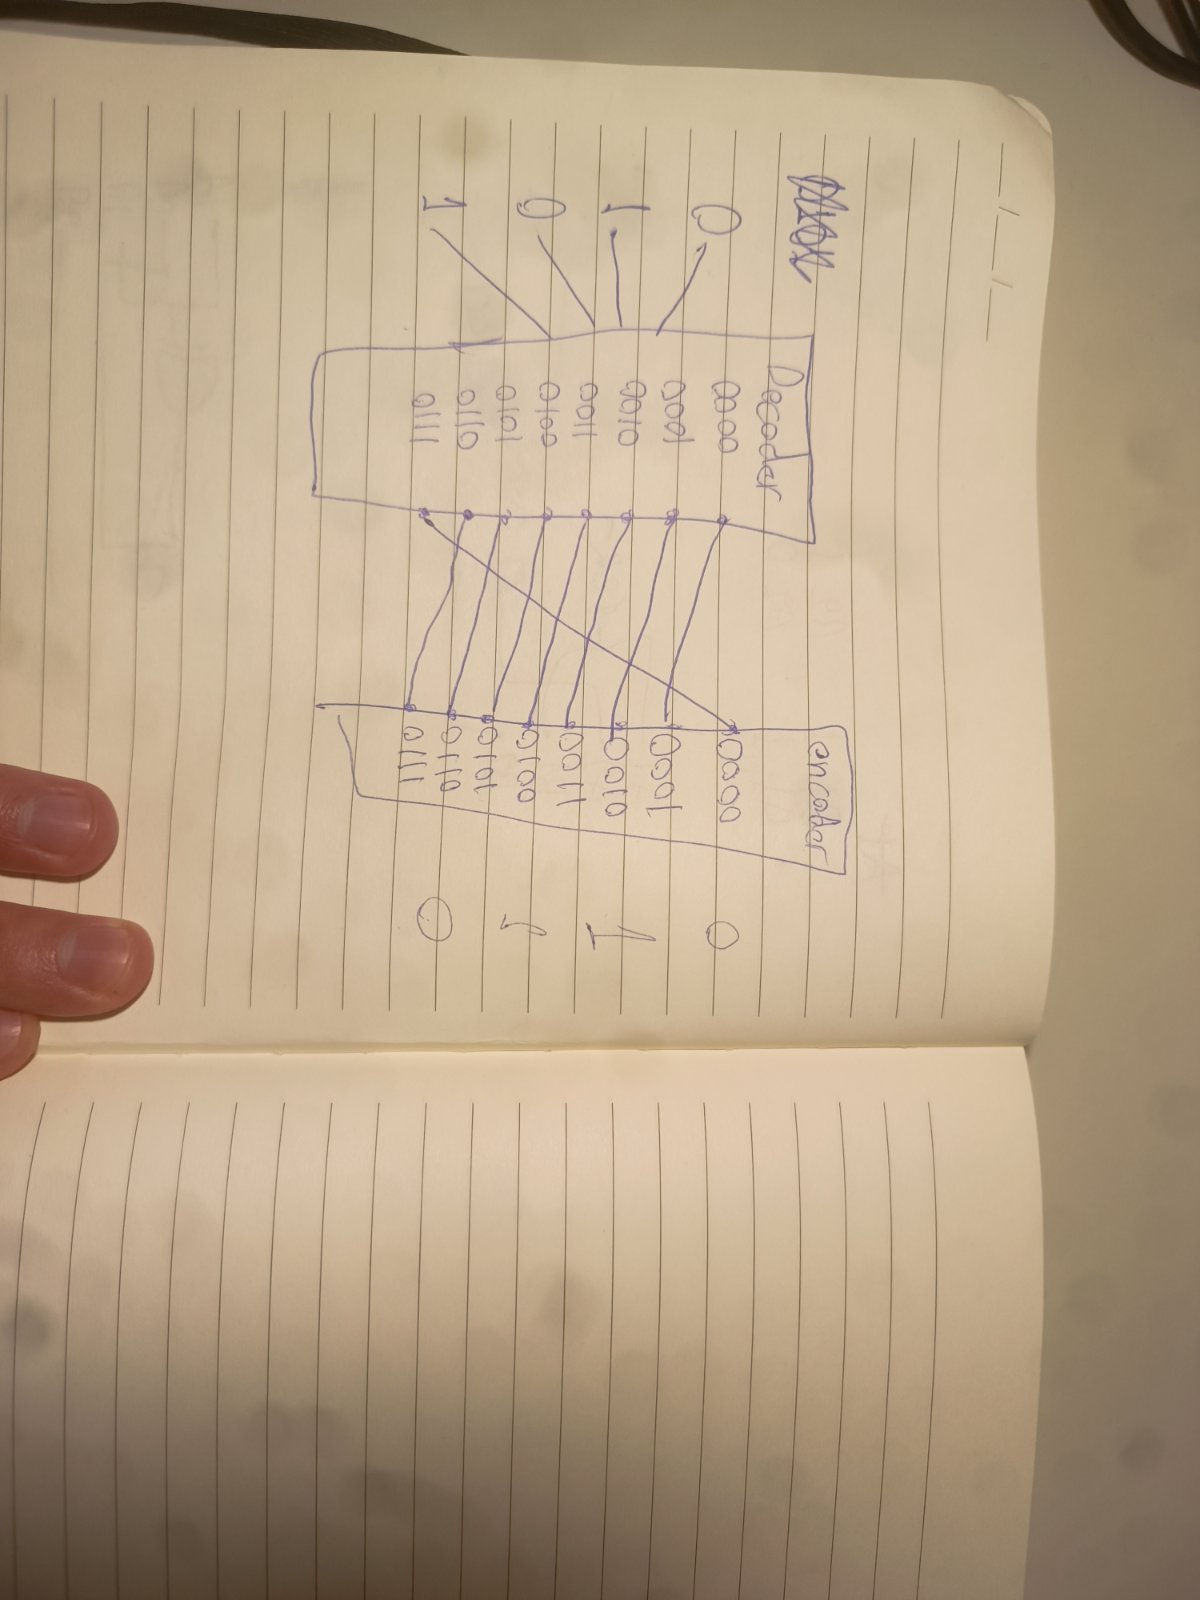
\includegraphics[width=\textwidth]{ex6.png}
		\caption{ex6}
    	\label{fig:ex6}
	\end{figure}
\end{solution}


\question Adding two numbers represented in scientific notation requires shifting floating points to make exponents equal before adding the fractions. \qpoints{15}
\\
Consider the following example:
\begin{itemize}
    \item Start with: $1.34 \cdot 10^3 + 2.1 \cdot 10^{-1}$
    \item Then, shift the decimal point of the smaller number to equalize the exponents:  
\(1.34 \cdot 10^3 + 0.00021 \cdot 10^3\)

\item Then add the fractions, and normalize the result if necessary:  
\(1.34021 \cdot 10^3\)
\end{itemize}

Assume we have two numbers \(N=14.25\) \(M=0.5\)  
\begin{enumerate}[label=\alph*)]
    \item Convert both numbers to IEEE floating point format.  
    \item Add the numbers using the described procedure (include implicit 1).  
    \item Normalize the result and convert it to IEEE format.  
\end{enumerate}

\begin{solution}
	 
	\begin{enumerate}[label=\alph*)]
		\item 
		\begin{align*}
		14.25 &= 0\ 10000010\ 11001000000000000000000 \\
		0.5 &= 0\ 01111110\ 00000000000000000000000
		\end{align*}
		\item
		\begin{itemize}
			\item Start with \(0\ 01111110\ 00000000000000000000000\).
			\item To convert \(2^{-1}\) to \(2^3\), we need to move the point by 4 positions. 
			\item The mantissa will become \(0.00010000000000000000000\) (but without the leading 0).
			\item The exponent will match that of 14.25.
		\end{itemize}
		Hence, we need to add:
		\[
		1.11001000000000000000000 + 0.00010000000000000000000 = 1.11011000000000000000000
		\]
		Since the result is positive and the exponent remains the same, the IEEE format will be:
		\[
		0\ 10000010\ 11011000000000000000000
		\]
	\end{enumerate}	
	
\end{solution}

\newpage
\question Design a circuit using logic gates to compare two 2-bit positive numbers. The output should be: \qpoints{15}
\begin{itemize}
    \item 10 if the first number is greater,
    \item 01 if the second number is greater,
    \item 00 if the two numbers are equal.
\end{itemize}

\begin{solution}
	\begin{figure}[H]
		\centering
		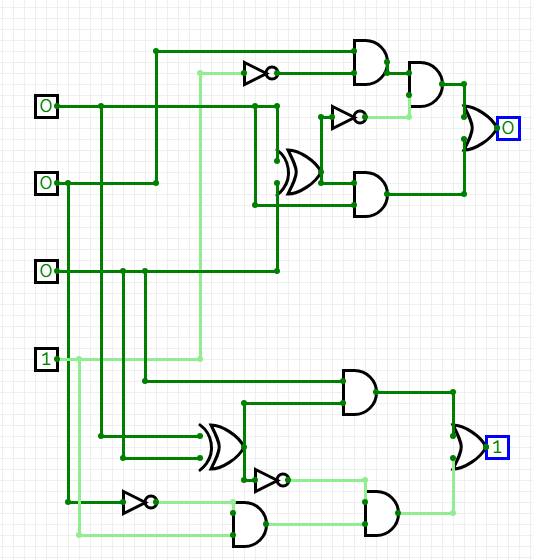
\includegraphics[width=\textwidth]{ex8.png}
		\caption{ex8}
    	\label{fig:ex8}
	\end{figure}
I split problem into the first bit and the second bit. the first output bit must be 1 only when the first number is greater. So i create a circuit for when the first number is greater. I start with xor because i split the task into when the first bits are the same and when they are not. If they are not the same then I make the output 1 when the first is the biggest (i just NOT the second bit and then AND both of them). If they are the same then i check for the second bits the same way. In the end I OR the 2 results because in case one of them outputs 1, it means that the above number is bigger. Then the same for the second output bit
\end{solution}



\end{questions}
\end{document}



